Activation functions play a central role in the artificial neural networks model, they are responsible for the non linearity of the model.
In the history of neural networks several activation functions have been proposed and used, in the following some of them are taken into consideration
underling the difference between them, with a special focus on their derivative expression.
A special class of activation function, is that of \textit{squashing} functions.

\begin{defn}
A function $f(\cdot):\mathbb{R}\rightarrow[a,b]$ with $a,b \in \mathbb{R}$ is said to be a \textit{squashing} function if it is not decreasing and 
\begin{align}
&\lim_{x \to +\infty} f(x) = b \\
&\lim_{x \to -\infty} f(x) = a 
\end{align}
\end{defn}
Step function, ramp function and all sigmoidal functions are all examples of squashing functions.

\begin{remark}
An important property of a \textit{squashing} function $\sigma(\cdot)$ is that
\begin{equation}
 \lim_{\alpha \to +\infty} \sigma(\alpha\cdot (x-\tau))= 
 \begin{cases}
    b \cdot \sigma_{\tau}(x) & \text{if $x> \tau $}\\
    a + \sigma_{\tau}(x) & \text{otherwise}
  \end{cases}
\end{equation}
being $\sigma_{\tau}$ the usual step function.
This property is extensively used in several proofs of the universal approximator property of neural networks. Roughly speaking we can say that \textit{squashing} functions act as step functions
at the limit; please note that this property has a practical use since inputs of activation functions are the weighted sum of some neurons output,
so activation function inputs can be arbitrarily big or small.
\end{remark}


\paragraph{Sigmoid}

\begin{align}
sigmoid(x)&= \frac{1}{1+e^{-x}}  \\ 
sigmoid'(x)&= sigmoid(x) \cdot (1-sigmoid(x))
\end{align}
As we can see from figure \ref{sigmoid_plot}, the sigmoid derivative has only one maximum in 0 where it assume value 0.25. Receding from 0, in both direction leads to regions where
the the derivative take zero value, such regions are called \textit{saturation} regions. If we happen to be in such regions, for a given neuron, we cannot learn anything since that neuron doesn't contribute
to the gradient.

\begin{figure}[ht]
  \centering
    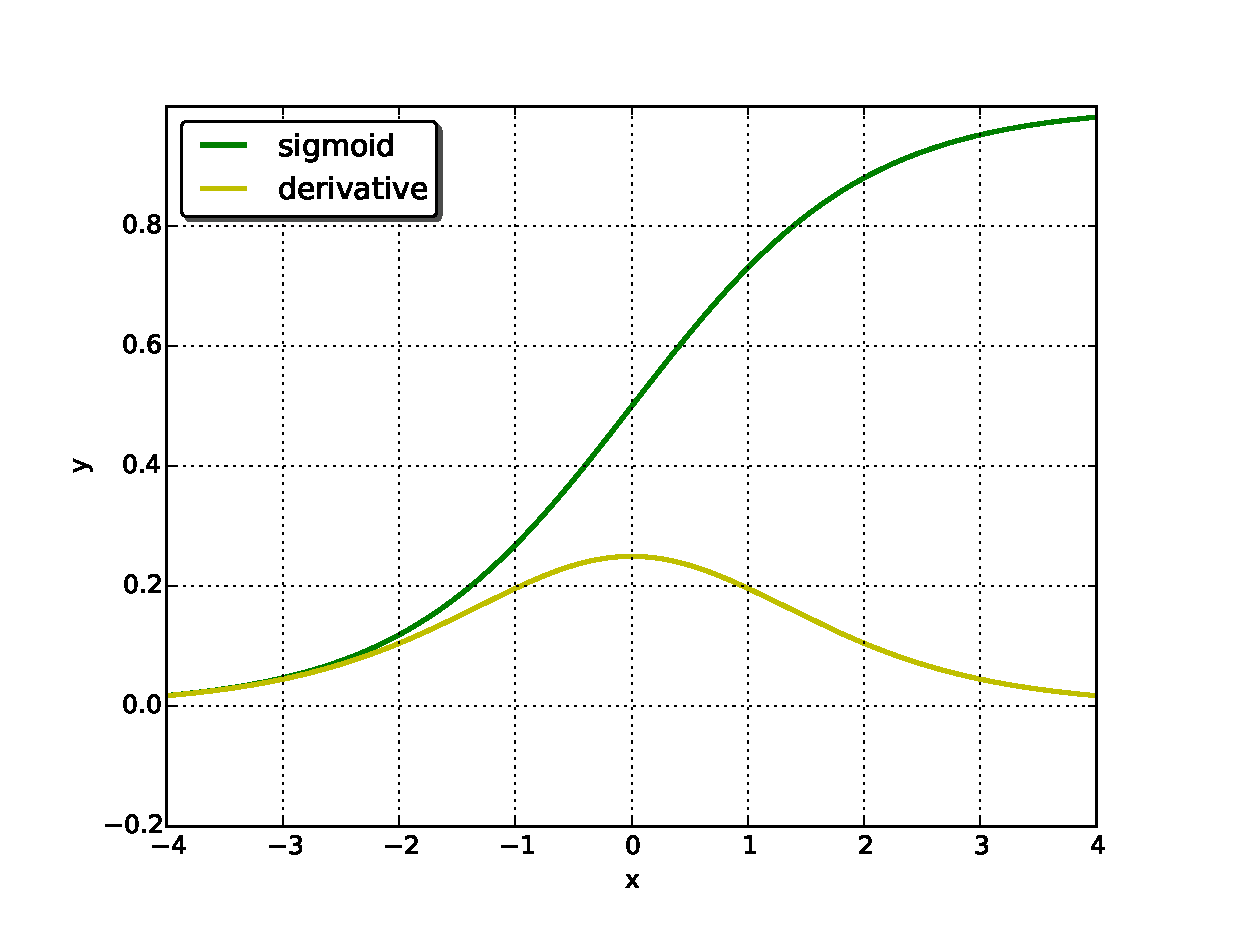
\includegraphics[width=0.9\textwidth]{sigmoid_and_deriv.eps}
  \caption{sigmoid and its derivative}
\label{sigmoid_plot}
\end{figure}

\paragraph{Tanh}
\begin{align}
 tanh(x)&=\frac{e^x-e^{-x}}{e^x+e^{-x}} \\
 tanh'(x)&= 1 - tanh^2(x)  
\end{align}
As we can see from figure \ref{tanh_plot} tanh (and it's derivative) have a behavior similar to the sigmoid one; Again we have two saturation region towards
infinity: that's typical of all squashing functions.



\begin{figure}[ht]
  \centering
    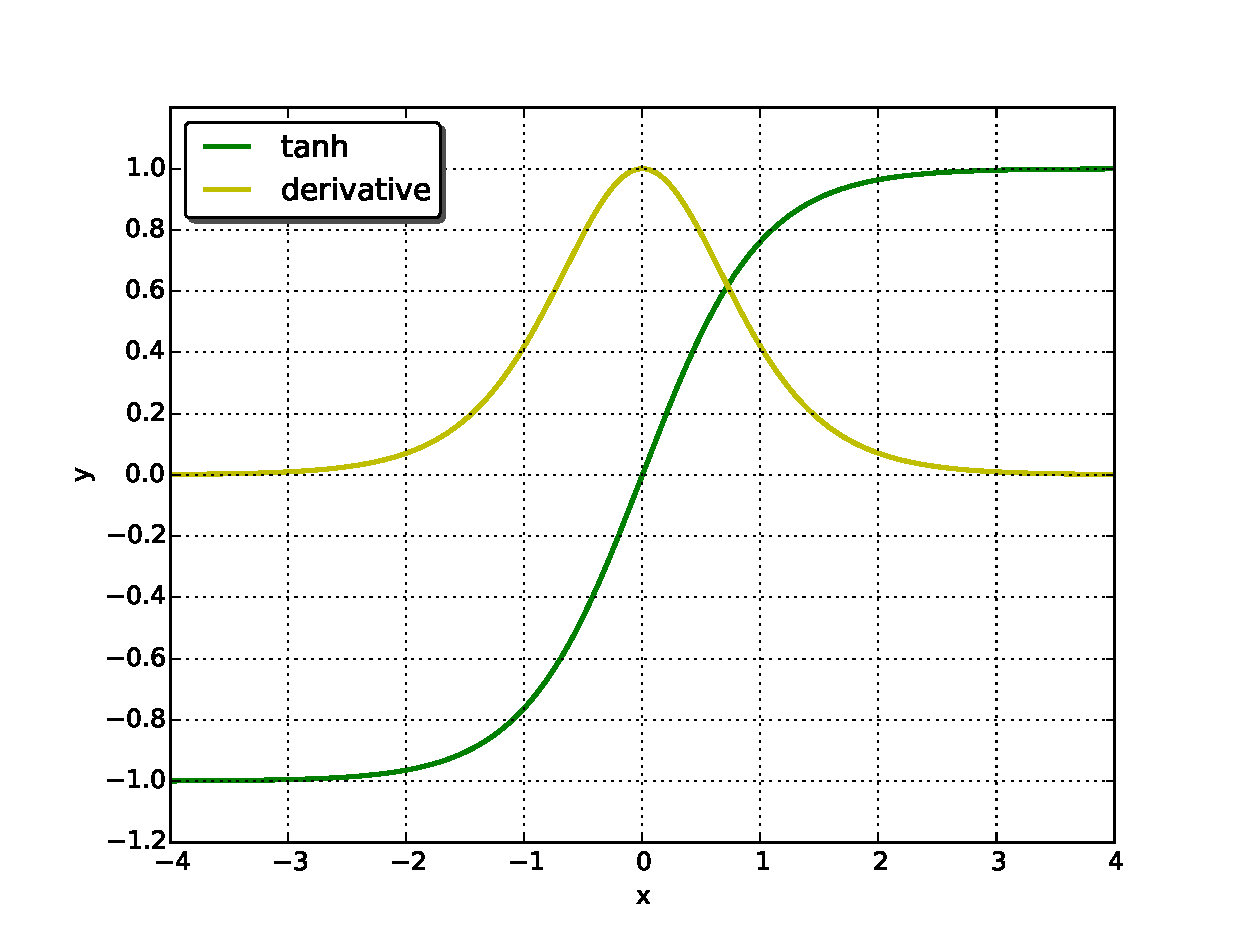
\includegraphics[width=0.9\textwidth]{tanh_and_deriv.eps}
  \caption{tanh and its derivative}
\label{tanh_plot}
\end{figure}



\paragraph{ReLU}


\begin{align}
  ReLU(x)&=\begin{cases}
    x & \text{if $x>0$}.\\
    0 & \text{otherwise}.
  \end{cases} \\ 
   ReLU'(x)&=\begin{cases}
    1 & \text{if $x>0$}.\\
    0 & \text{otherwise}.
  \end{cases}
\end{align}
ReLU is a bit different from other activation function seen so far: the main difference is that's it's not a squashing function.
As we can see from figure \ref{relu_plot}, ReLU's derivative is the step function; it has only one \textit{saturation} region $(-\infty, 0]$ and a region in which is always takes value 1, $(0,+\infty]$
This leads to the fact that we cannot learn to \textit{turn on} a switched off neuron ($x<0$), but we have no \textit{saturation} region toward infinity.
The constancy of the derivative in the \textit{active} region is a distinctive property of ReLU which plays an important role in the \textit{vanishing gradient} problem too, as it's explained in the relative
section.

\begin{figure}[ht]
  \centering
    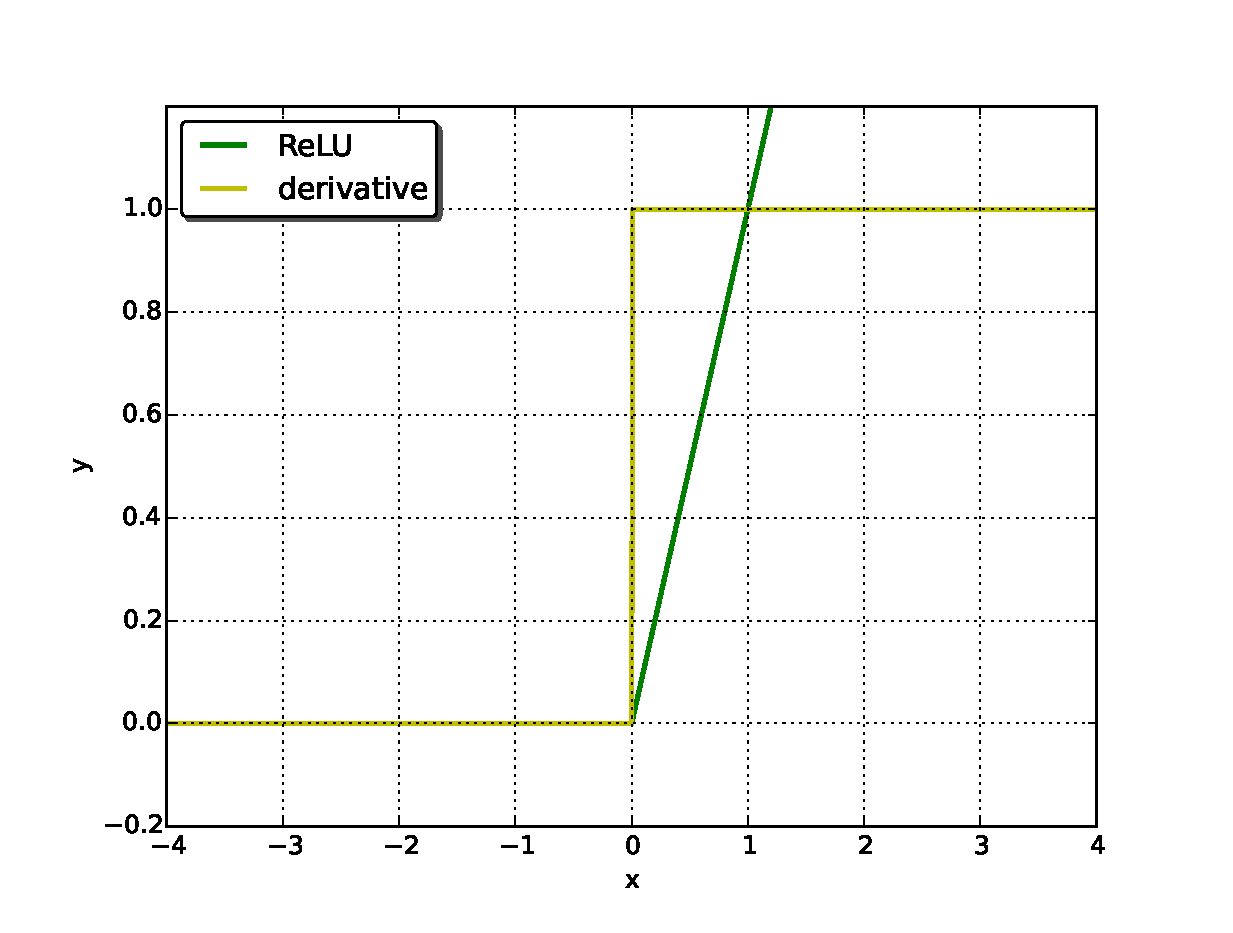
\includegraphics[width=0.9\textwidth]{relu_and_deriv.eps}
  \caption{ReLU and its derivative}
\label{relu_plot}
\end{figure}
